% Options for packages loaded elsewhere
\PassOptionsToPackage{unicode}{hyperref}
\PassOptionsToPackage{hyphens}{url}
%
\documentclass[
]{article}
\usepackage{lmodern}
\usepackage{amssymb,amsmath}
\usepackage{ifxetex,ifluatex}
\ifnum 0\ifxetex 1\fi\ifluatex 1\fi=0 % if pdftex
  \usepackage[T1]{fontenc}
  \usepackage[utf8]{inputenc}
  \usepackage{textcomp} % provide euro and other symbols
\else % if luatex or xetex
  \usepackage{unicode-math}
  \defaultfontfeatures{Scale=MatchLowercase}
  \defaultfontfeatures[\rmfamily]{Ligatures=TeX,Scale=1}
\fi
% Use upquote if available, for straight quotes in verbatim environments
\IfFileExists{upquote.sty}{\usepackage{upquote}}{}
\IfFileExists{microtype.sty}{% use microtype if available
  \usepackage[]{microtype}
  \UseMicrotypeSet[protrusion]{basicmath} % disable protrusion for tt fonts
}{}
\makeatletter
\@ifundefined{KOMAClassName}{% if non-KOMA class
  \IfFileExists{parskip.sty}{%
    \usepackage{parskip}
  }{% else
    \setlength{\parindent}{0pt}
    \setlength{\parskip}{6pt plus 2pt minus 1pt}}
}{% if KOMA class
  \KOMAoptions{parskip=half}}
\makeatother
\usepackage{xcolor}
\IfFileExists{xurl.sty}{\usepackage{xurl}}{} % add URL line breaks if available
\IfFileExists{bookmark.sty}{\usepackage{bookmark}}{\usepackage{hyperref}}
\hypersetup{
  pdftitle={Reproducible Research},
  pdfauthor={Chiranthi},
  hidelinks,
  pdfcreator={LaTeX via pandoc}}
\urlstyle{same} % disable monospaced font for URLs
\usepackage[margin=1in]{geometry}
\usepackage{color}
\usepackage{fancyvrb}
\newcommand{\VerbBar}{|}
\newcommand{\VERB}{\Verb[commandchars=\\\{\}]}
\DefineVerbatimEnvironment{Highlighting}{Verbatim}{commandchars=\\\{\}}
% Add ',fontsize=\small' for more characters per line
\usepackage{framed}
\definecolor{shadecolor}{RGB}{248,248,248}
\newenvironment{Shaded}{\begin{snugshade}}{\end{snugshade}}
\newcommand{\AlertTok}[1]{\textcolor[rgb]{0.94,0.16,0.16}{#1}}
\newcommand{\AnnotationTok}[1]{\textcolor[rgb]{0.56,0.35,0.01}{\textbf{\textit{#1}}}}
\newcommand{\AttributeTok}[1]{\textcolor[rgb]{0.77,0.63,0.00}{#1}}
\newcommand{\BaseNTok}[1]{\textcolor[rgb]{0.00,0.00,0.81}{#1}}
\newcommand{\BuiltInTok}[1]{#1}
\newcommand{\CharTok}[1]{\textcolor[rgb]{0.31,0.60,0.02}{#1}}
\newcommand{\CommentTok}[1]{\textcolor[rgb]{0.56,0.35,0.01}{\textit{#1}}}
\newcommand{\CommentVarTok}[1]{\textcolor[rgb]{0.56,0.35,0.01}{\textbf{\textit{#1}}}}
\newcommand{\ConstantTok}[1]{\textcolor[rgb]{0.00,0.00,0.00}{#1}}
\newcommand{\ControlFlowTok}[1]{\textcolor[rgb]{0.13,0.29,0.53}{\textbf{#1}}}
\newcommand{\DataTypeTok}[1]{\textcolor[rgb]{0.13,0.29,0.53}{#1}}
\newcommand{\DecValTok}[1]{\textcolor[rgb]{0.00,0.00,0.81}{#1}}
\newcommand{\DocumentationTok}[1]{\textcolor[rgb]{0.56,0.35,0.01}{\textbf{\textit{#1}}}}
\newcommand{\ErrorTok}[1]{\textcolor[rgb]{0.64,0.00,0.00}{\textbf{#1}}}
\newcommand{\ExtensionTok}[1]{#1}
\newcommand{\FloatTok}[1]{\textcolor[rgb]{0.00,0.00,0.81}{#1}}
\newcommand{\FunctionTok}[1]{\textcolor[rgb]{0.00,0.00,0.00}{#1}}
\newcommand{\ImportTok}[1]{#1}
\newcommand{\InformationTok}[1]{\textcolor[rgb]{0.56,0.35,0.01}{\textbf{\textit{#1}}}}
\newcommand{\KeywordTok}[1]{\textcolor[rgb]{0.13,0.29,0.53}{\textbf{#1}}}
\newcommand{\NormalTok}[1]{#1}
\newcommand{\OperatorTok}[1]{\textcolor[rgb]{0.81,0.36,0.00}{\textbf{#1}}}
\newcommand{\OtherTok}[1]{\textcolor[rgb]{0.56,0.35,0.01}{#1}}
\newcommand{\PreprocessorTok}[1]{\textcolor[rgb]{0.56,0.35,0.01}{\textit{#1}}}
\newcommand{\RegionMarkerTok}[1]{#1}
\newcommand{\SpecialCharTok}[1]{\textcolor[rgb]{0.00,0.00,0.00}{#1}}
\newcommand{\SpecialStringTok}[1]{\textcolor[rgb]{0.31,0.60,0.02}{#1}}
\newcommand{\StringTok}[1]{\textcolor[rgb]{0.31,0.60,0.02}{#1}}
\newcommand{\VariableTok}[1]{\textcolor[rgb]{0.00,0.00,0.00}{#1}}
\newcommand{\VerbatimStringTok}[1]{\textcolor[rgb]{0.31,0.60,0.02}{#1}}
\newcommand{\WarningTok}[1]{\textcolor[rgb]{0.56,0.35,0.01}{\textbf{\textit{#1}}}}
\usepackage{graphicx,grffile}
\makeatletter
\def\maxwidth{\ifdim\Gin@nat@width>\linewidth\linewidth\else\Gin@nat@width\fi}
\def\maxheight{\ifdim\Gin@nat@height>\textheight\textheight\else\Gin@nat@height\fi}
\makeatother
% Scale images if necessary, so that they will not overflow the page
% margins by default, and it is still possible to overwrite the defaults
% using explicit options in \includegraphics[width, height, ...]{}
\setkeys{Gin}{width=\maxwidth,height=\maxheight,keepaspectratio}
% Set default figure placement to htbp
\makeatletter
\def\fps@figure{htbp}
\makeatother
\setlength{\emergencystretch}{3em} % prevent overfull lines
\providecommand{\tightlist}{%
  \setlength{\itemsep}{0pt}\setlength{\parskip}{0pt}}
\setcounter{secnumdepth}{-\maxdimen} % remove section numbering

\title{Reproducible Research}
\author{Chiranthi}
\date{7/1/2020}

\begin{document}
\maketitle

\hypertarget{peer-graded-assignment-course-project-1}{%
\subsection{Peer-graded Assignment: Course Project
1}\label{peer-graded-assignment-course-project-1}}

This assignment makes use of data from a personal activity monitoring
device. This device collects data at 5 minute intervals through out the
day. The data consists of two months of data from an anonymous
individual collected during the months of October and November, 2012 and
include the number of steps taken in 5 minute intervals each day.

\hypertarget{loading-packages}{%
\subsection{Loading Packages}\label{loading-packages}}

\begin{verbatim}
## Warning: package 'dplyr' was built under R version 3.5.3
\end{verbatim}

\begin{verbatim}
## 
## Attaching package: 'dplyr'
\end{verbatim}

\begin{verbatim}
## The following objects are masked from 'package:stats':
## 
##     filter, lag
\end{verbatim}

\begin{verbatim}
## The following objects are masked from 'package:base':
## 
##     intersect, setdiff, setequal, union
\end{verbatim}

\begin{verbatim}
## Warning: package 'lubridate' was built under R version 3.5.3
\end{verbatim}

\begin{verbatim}
## 
## Attaching package: 'lubridate'
\end{verbatim}

\begin{verbatim}
## The following objects are masked from 'package:dplyr':
## 
##     intersect, setdiff, union
\end{verbatim}

\begin{verbatim}
## The following objects are masked from 'package:base':
## 
##     date, intersect, setdiff, union
\end{verbatim}

\begin{verbatim}
## Warning: package 'data.table' was built under R version 3.5.3
\end{verbatim}

\begin{verbatim}
## 
## Attaching package: 'data.table'
\end{verbatim}

\begin{verbatim}
## The following objects are masked from 'package:lubridate':
## 
##     hour, isoweek, mday, minute, month, quarter, second, wday, week,
##     yday, year
\end{verbatim}

\begin{verbatim}
## The following objects are masked from 'package:dplyr':
## 
##     between, first, last
\end{verbatim}

\hypertarget{loading-data}{%
\subsection{lOading Data}\label{loading-data}}

\begin{Shaded}
\begin{Highlighting}[]
\NormalTok{fileUrl <-}\StringTok{ "https://d396qusza40orc.cloudfront.net/repdata%2Fdata%2Factivity.zip"}
\KeywordTok{download.file}\NormalTok{(fileUrl, }\DataTypeTok{destfile =} \KeywordTok{paste0}\NormalTok{(}\KeywordTok{getwd}\NormalTok{(), }\StringTok{'/repdata%2Fdata%2Factivity.zip'}\NormalTok{), }\DataTypeTok{method =} \StringTok{"curl"}\NormalTok{)}
\KeywordTok{unzip}\NormalTok{(}\StringTok{"repdata%2Fdata%2Factivity.zip"}\NormalTok{,}\DataTypeTok{exdir =} \StringTok{"data"}\NormalTok{)}

\NormalTok{activitydata <-}\StringTok{ }\NormalTok{data.table}\OperatorTok{::}\KeywordTok{fread}\NormalTok{(}\DataTypeTok{input =} \StringTok{"data/activity.csv"}\NormalTok{)}
\end{Highlighting}
\end{Shaded}

\hypertarget{getting-some-insights-about-data}{%
\subsection{Getting some insights about
data}\label{getting-some-insights-about-data}}

\begin{Shaded}
\begin{Highlighting}[]
\KeywordTok{head}\NormalTok{(activitydata)}
\end{Highlighting}
\end{Shaded}

\begin{verbatim}
##    steps       date interval
## 1:    NA 2012-10-01        0
## 2:    NA 2012-10-01        5
## 3:    NA 2012-10-01       10
## 4:    NA 2012-10-01       15
## 5:    NA 2012-10-01       20
## 6:    NA 2012-10-01       25
\end{verbatim}

\begin{Shaded}
\begin{Highlighting}[]
\KeywordTok{tail}\NormalTok{(activitydata)}
\end{Highlighting}
\end{Shaded}

\begin{verbatim}
##    steps       date interval
## 1:    NA 2012-11-30     2330
## 2:    NA 2012-11-30     2335
## 3:    NA 2012-11-30     2340
## 4:    NA 2012-11-30     2345
## 5:    NA 2012-11-30     2350
## 6:    NA 2012-11-30     2355
\end{verbatim}

\begin{Shaded}
\begin{Highlighting}[]
\KeywordTok{glimpse}\NormalTok{(activitydata)}
\end{Highlighting}
\end{Shaded}

\begin{verbatim}
## Rows: 17,568
## Columns: 3
## $ steps    <int> NA, NA, NA, NA, NA, NA, NA, NA, NA, NA, NA, NA, NA, NA, NA...
## $ date     <chr> "2012-10-01", "2012-10-01", "2012-10-01", "2012-10-01", "2...
## $ interval <int> 0, 5, 10, 15, 20, 25, 30, 35, 40, 45, 50, 55, 100, 105, 11...
\end{verbatim}

\begin{Shaded}
\begin{Highlighting}[]
\KeywordTok{str}\NormalTok{(activitydata)}
\end{Highlighting}
\end{Shaded}

\begin{verbatim}
## Classes 'data.table' and 'data.frame':   17568 obs. of  3 variables:
##  $ steps   : int  NA NA NA NA NA NA NA NA NA NA ...
##  $ date    : chr  "2012-10-01" "2012-10-01" "2012-10-01" "2012-10-01" ...
##  $ interval: int  0 5 10 15 20 25 30 35 40 45 ...
##  - attr(*, ".internal.selfref")=<externalptr>
\end{verbatim}

\hypertarget{converting-date-column-to-date-data-type}{%
\subsection{converting date column to date data
type}\label{converting-date-column-to-date-data-type}}

\begin{Shaded}
\begin{Highlighting}[]
\NormalTok{activitydata}\OperatorTok{$}\NormalTok{Date <-}\StringTok{ }\KeywordTok{as.Date}\NormalTok{(}\KeywordTok{paste0}\NormalTok{(}\KeywordTok{as.character}\NormalTok{(activitydata}\OperatorTok{$}\NormalTok{date), }\DataTypeTok{format =} \StringTok{"ymd"}\NormalTok{))}
\end{Highlighting}
\end{Shaded}

\hypertarget{histogram-of-the-total-number-of-steps-taken-each-day}{%
\subsection{Histogram of the total number of steps taken each
day}\label{histogram-of-the-total-number-of-steps-taken-each-day}}

\begin{Shaded}
\begin{Highlighting}[]
\NormalTok{Steps <-}\StringTok{ }\NormalTok{activitydata }\OperatorTok
\StringTok{  }\KeywordTok{group_by}\NormalTok{(Date) }\OperatorTok
\StringTok{  }\KeywordTok{summarise}\NormalTok{( }\DataTypeTok{Total =} \KeywordTok{sum}\NormalTok{(steps), }\DataTypeTok{na.rm =} \OtherTok{TRUE}\NormalTok{)}

\CommentTok{# Drawing the histogram }
\KeywordTok{ggplot}\NormalTok{(Steps)}\OperatorTok{+}
\StringTok{  }\KeywordTok{geom_histogram}\NormalTok{(}\KeywordTok{aes}\NormalTok{(}\DataTypeTok{x =}\NormalTok{ Total), }\DataTypeTok{binwidth =} \DecValTok{1000}\NormalTok{) }\OperatorTok{+}
\StringTok{  }\KeywordTok{labs}\NormalTok{(}\DataTypeTok{title =} \StringTok{"Daily Steps"}\NormalTok{, }\DataTypeTok{x =} \StringTok{"Steps"}\NormalTok{, }\DataTypeTok{y =} \StringTok{"Frequency"}\NormalTok{)}
\end{Highlighting}
\end{Shaded}

\begin{verbatim}
## Warning: Removed 8 rows containing non-finite values (stat_bin).
\end{verbatim}

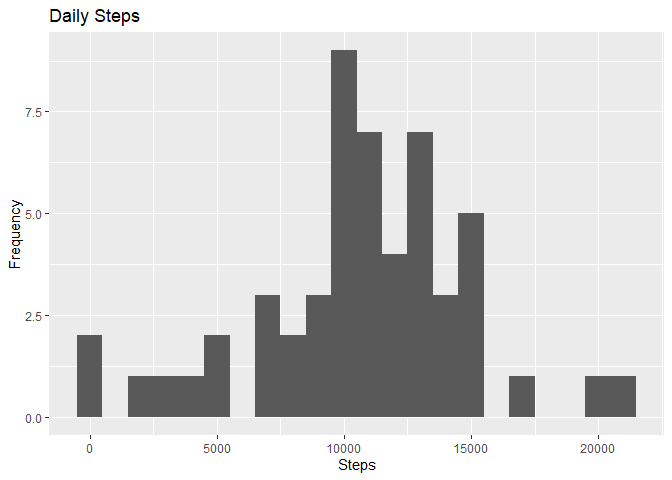
\includegraphics{Peer-graded_Assignment_files/figure-latex/unnamed-chunk-4-1.pdf}

\hypertarget{mean-and-median-number-of-steps-taken-each-day}{%
\subsection{Mean and median number of steps taken each
day}\label{mean-and-median-number-of-steps-taken-each-day}}

\begin{Shaded}
\begin{Highlighting}[]
\NormalTok{rawsteps_mean <-}\StringTok{ }\KeywordTok{mean}\NormalTok{(Steps}\OperatorTok{$}\NormalTok{Total, }\DataTypeTok{na.rm=}\OtherTok{TRUE}\NormalTok{)}
\NormalTok{rawsteps_median <-}\StringTok{ }\KeywordTok{median}\NormalTok{(Steps}\OperatorTok{$}\NormalTok{Total, }\DataTypeTok{na.rm=}\OtherTok{TRUE}\NormalTok{)}
\KeywordTok{print}\NormalTok{(}\KeywordTok{paste}\NormalTok{(}\StringTok{"The mean steps per day is: "}\NormalTok{, rawsteps_mean))}
\end{Highlighting}
\end{Shaded}

\begin{verbatim}
## [1] "The mean steps per day is:  10766.1886792453"
\end{verbatim}

\begin{Shaded}
\begin{Highlighting}[]
\KeywordTok{print}\NormalTok{(}\KeywordTok{paste}\NormalTok{(}\StringTok{"The median steps per day is: "}\NormalTok{, rawsteps_median))}
\end{Highlighting}
\end{Shaded}

\begin{verbatim}
## [1] "The median steps per day is:  10765"
\end{verbatim}

\hypertarget{time-series-plot-of-the-average-number-of-steps-taken}{%
\subsection{Time series plot of the average number of steps
taken}\label{time-series-plot-of-the-average-number-of-steps-taken}}

\begin{Shaded}
\begin{Highlighting}[]
\NormalTok{IntervalDT <-}\StringTok{ }\NormalTok{activitydata[, }\KeywordTok{c}\NormalTok{(}\KeywordTok{lapply}\NormalTok{(.SD, mean, }\DataTypeTok{na.rm =} \OtherTok{TRUE}\NormalTok{)), .SDcols =}\StringTok{ }\KeywordTok{c}\NormalTok{(}\StringTok{"steps"}\NormalTok{), by =}\StringTok{ }\NormalTok{.(interval)] }

\KeywordTok{ggplot}\NormalTok{(IntervalDT, }\KeywordTok{aes}\NormalTok{(}\DataTypeTok{x =}\NormalTok{ interval , }\DataTypeTok{y =}\NormalTok{ steps)) }\OperatorTok{+}\StringTok{ }\KeywordTok{geom_line}\NormalTok{(}\DataTypeTok{color=}\StringTok{"blue"}\NormalTok{, }\DataTypeTok{size=}\DecValTok{1}\NormalTok{) }\OperatorTok{+}\StringTok{ }\KeywordTok{labs}\NormalTok{(}\DataTypeTok{title =} \StringTok{"Avg. Daily Steps"}\NormalTok{, }\DataTypeTok{x =} \StringTok{"Interval"}\NormalTok{, }\DataTypeTok{y =} \StringTok{"Avg. Steps per day"}\NormalTok{)}
\end{Highlighting}
\end{Shaded}

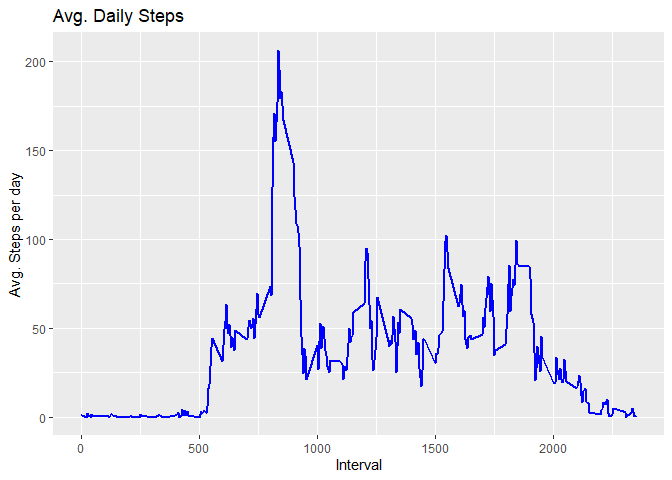
\includegraphics{Peer-graded_Assignment_files/figure-latex/unnamed-chunk-6-1.pdf}

\hypertarget{which-5-minute-interval-on-average-across-all-the-days-in-the-dataset-contains-the-maximum-number-of-steps}{%
\subsection{Which 5-minute interval, on average across all the days in
the dataset, contains the maximum number of
steps?}\label{which-5-minute-interval-on-average-across-all-the-days-in-the-dataset-contains-the-maximum-number-of-steps}}

\begin{Shaded}
\begin{Highlighting}[]
\NormalTok{IntervalDT[steps }\OperatorTok{==}\StringTok{ }\KeywordTok{max}\NormalTok{(steps), .(}\DataTypeTok{max_interval =}\NormalTok{ interval)]}
\end{Highlighting}
\end{Shaded}

\begin{verbatim}
##    max_interval
## 1:          835
\end{verbatim}

\hypertarget{calculate-and-report-the-total-number-of-missing-values-in-the-dataset-i.e.-the-total-number-of-rows-with-s}{%
\subsection{Calculate and report the total number of missing values in
the dataset (i.e.~the total number of rows with
????????s)}\label{calculate-and-report-the-total-number-of-missing-values-in-the-dataset-i.e.-the-total-number-of-rows-with-s}}

\begin{Shaded}
\begin{Highlighting}[]
\NormalTok{activitydata[}\KeywordTok{is.na}\NormalTok{(steps), .N ]}
\end{Highlighting}
\end{Shaded}

\begin{verbatim}
## [1] 2304
\end{verbatim}

Code to describe and show a strategy for imputing missing data.

\begin{Shaded}
\begin{Highlighting}[]
\CommentTok{# Filling in missing values with median of dataset. }
\NormalTok{activitydata[}\KeywordTok{is.na}\NormalTok{(steps), }\StringTok{"steps"}\NormalTok{] <-}\StringTok{ }\NormalTok{activitydata[, }\KeywordTok{c}\NormalTok{(}\KeywordTok{lapply}\NormalTok{(.SD, median, }\DataTypeTok{na.rm =} \OtherTok{TRUE}\NormalTok{)), .SDcols =}\StringTok{ }\KeywordTok{c}\NormalTok{(}\StringTok{"steps"}\NormalTok{)]}
\end{Highlighting}
\end{Shaded}

Creating a new dataset that is equal to the original dataset but with
the missing data filled in.

\begin{Shaded}
\begin{Highlighting}[]
\NormalTok{data.table}\OperatorTok{::}\KeywordTok{fwrite}\NormalTok{(}\DataTypeTok{x =}\NormalTok{ activitydata, }\DataTypeTok{file =} \StringTok{"data/tidyData.csv"}\NormalTok{, }\DataTypeTok{quote =} \OtherTok{FALSE}\NormalTok{)}
\end{Highlighting}
\end{Shaded}

Making a histogram of the total number of steps taken each day and
calculate and report the mean and median total number of steps taken per
day. Do these values differ from the estimates from the first part of
the assignment? What is the impact of imputing missing data on the
estimates of the total daily number of steps?

\begin{Shaded}
\begin{Highlighting}[]
\CommentTok{# total number of steps taken per day}
\NormalTok{Total_Steps <-}\StringTok{ }\NormalTok{activitydata[, }\KeywordTok{c}\NormalTok{(}\KeywordTok{lapply}\NormalTok{(.SD, sum)), .SDcols =}\StringTok{ }\KeywordTok{c}\NormalTok{(}\StringTok{"steps"}\NormalTok{), by =}\StringTok{ }\NormalTok{.(date)] }

\CommentTok{# mean and median total number of steps taken per day}
\NormalTok{Total_Steps[, .(}\DataTypeTok{Mean_Steps =} \KeywordTok{mean}\NormalTok{(steps), }\DataTypeTok{Median_Steps =} \KeywordTok{median}\NormalTok{(steps))]}
\end{Highlighting}
\end{Shaded}

\begin{verbatim}
##    Mean_Steps Median_Steps
## 1:    9354.23        10395
\end{verbatim}

\begin{Shaded}
\begin{Highlighting}[]
\KeywordTok{ggplot}\NormalTok{(Total_Steps, }\KeywordTok{aes}\NormalTok{(}\DataTypeTok{x =}\NormalTok{ steps)) }\OperatorTok{+}\StringTok{ }\KeywordTok{geom_histogram}\NormalTok{(}\DataTypeTok{fill =} \StringTok{"blue"}\NormalTok{, }\DataTypeTok{binwidth =} \DecValTok{1000}\NormalTok{) }\OperatorTok{+}\StringTok{ }\KeywordTok{labs}\NormalTok{(}\DataTypeTok{title =} \StringTok{"Daily Steps"}\NormalTok{, }\DataTypeTok{x =} \StringTok{"Steps"}\NormalTok{, }\DataTypeTok{y =} \StringTok{"Frequency"}\NormalTok{)}
\end{Highlighting}
\end{Shaded}

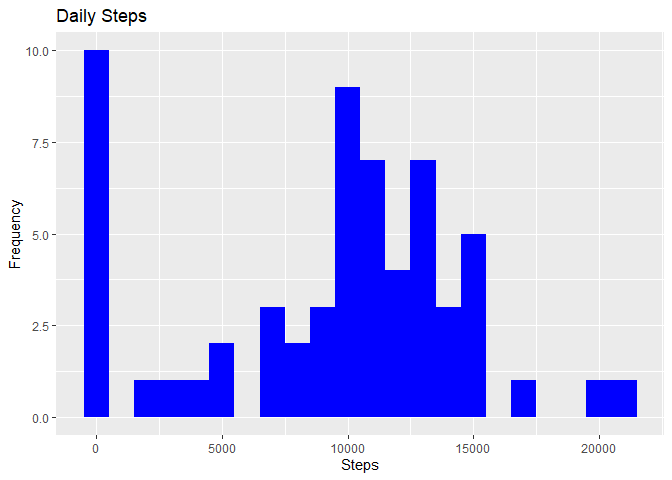
\includegraphics{Peer-graded_Assignment_files/figure-latex/unnamed-chunk-11-1.pdf}

\hypertarget{are-there-differences-in-activity-patterns-between-weekdays-and-weekends}{%
\subsection{Are there differences in activity patterns between weekdays
and
weekends?}\label{are-there-differences-in-activity-patterns-between-weekdays-and-weekends}}

Create a new factor variable in the dataset with two levels -
``weekday'' and ``weekend'' indicating whether a given date is a weekday
or weekend day.

\begin{Shaded}
\begin{Highlighting}[]
\CommentTok{# Just recreating activitydata from scratch then making the new factor variable. (No need to, just want to be clear on what the entire process is.) }
\NormalTok{activitydata <-}\StringTok{ }\NormalTok{data.table}\OperatorTok{::}\KeywordTok{fread}\NormalTok{(}\DataTypeTok{input =} \StringTok{"data/activity.csv"}\NormalTok{)}
\NormalTok{activitydata[, date }\OperatorTok{:}\ErrorTok{=}\StringTok{ }\KeywordTok{as.POSIXct}\NormalTok{(date, }\DataTypeTok{format =} \StringTok{"%Y-%m-%d"}\NormalTok{)]}
\NormalTok{activitydata[, }\StringTok{`}\DataTypeTok{Day of Week}\StringTok{`}\OperatorTok{:}\ErrorTok{=}\StringTok{ }\KeywordTok{weekdays}\NormalTok{(}\DataTypeTok{x =}\NormalTok{ date)]}
\NormalTok{activitydata[}\KeywordTok{grepl}\NormalTok{(}\DataTypeTok{pattern =} \StringTok{"Monday|Tuesday|Wednesday|Thursday|Friday"}\NormalTok{, }\DataTypeTok{x =} \StringTok{`}\DataTypeTok{Day of Week}\StringTok{`}\NormalTok{), }\StringTok{"weekday or weekend"}\NormalTok{] <-}\StringTok{ "weekday"}
\NormalTok{activitydata[}\KeywordTok{grepl}\NormalTok{(}\DataTypeTok{pattern =} \StringTok{"Saturday|Sunday"}\NormalTok{, }\DataTypeTok{x =} \StringTok{`}\DataTypeTok{Day of Week}\StringTok{`}\NormalTok{), }\StringTok{"weekday or weekend"}\NormalTok{] <-}\StringTok{ "weekend"}
\NormalTok{activitydata[, }\StringTok{`}\DataTypeTok{weekday or weekend}\StringTok{`} \OperatorTok{:}\ErrorTok{=}\StringTok{ }\KeywordTok{as.factor}\NormalTok{(}\StringTok{`}\DataTypeTok{weekday or weekend}\StringTok{`}\NormalTok{)]}
\KeywordTok{head}\NormalTok{(activitydata, }\DecValTok{10}\NormalTok{)}
\end{Highlighting}
\end{Shaded}

\begin{verbatim}
##     steps       date interval Day of Week weekday or weekend
##  1:    NA 2012-10-01        0      Monday            weekday
##  2:    NA 2012-10-01        5      Monday            weekday
##  3:    NA 2012-10-01       10      Monday            weekday
##  4:    NA 2012-10-01       15      Monday            weekday
##  5:    NA 2012-10-01       20      Monday            weekday
##  6:    NA 2012-10-01       25      Monday            weekday
##  7:    NA 2012-10-01       30      Monday            weekday
##  8:    NA 2012-10-01       35      Monday            weekday
##  9:    NA 2012-10-01       40      Monday            weekday
## 10:    NA 2012-10-01       45      Monday            weekday
\end{verbatim}

Make a panel plot containing a time series plot (i.e.~???????????????? =
``????'') of the 5-minute interval (x-axis) and the average number of
steps taken, averaged across all weekday days or weekend days (y-axis).
See the README file in the GitHub repository to see an example of what
this plot should look like using simulated data.

\begin{Shaded}
\begin{Highlighting}[]
\NormalTok{activitydata[}\KeywordTok{is.na}\NormalTok{(steps), }\StringTok{"steps"}\NormalTok{] <-}\StringTok{ }\NormalTok{activitydata[, }\KeywordTok{c}\NormalTok{(}\KeywordTok{lapply}\NormalTok{(.SD, median, }\DataTypeTok{na.rm =} \OtherTok{TRUE}\NormalTok{)), .SDcols =}\StringTok{ }\KeywordTok{c}\NormalTok{(}\StringTok{"steps"}\NormalTok{)]}
\NormalTok{IntervalDT <-}\StringTok{ }\NormalTok{activitydata[, }\KeywordTok{c}\NormalTok{(}\KeywordTok{lapply}\NormalTok{(.SD, mean, }\DataTypeTok{na.rm =} \OtherTok{TRUE}\NormalTok{)), .SDcols =}\StringTok{ }\KeywordTok{c}\NormalTok{(}\StringTok{"steps"}\NormalTok{), by =}\StringTok{ }\NormalTok{.(interval, }\StringTok{`}\DataTypeTok{weekday or weekend}\StringTok{`}\NormalTok{)] }

\KeywordTok{ggplot}\NormalTok{(IntervalDT , }\KeywordTok{aes}\NormalTok{(}\DataTypeTok{x =}\NormalTok{ interval , }\DataTypeTok{y =}\NormalTok{ steps, }\DataTypeTok{color=}\StringTok{`}\DataTypeTok{weekday or weekend}\StringTok{`}\NormalTok{)) }\OperatorTok{+}\StringTok{ }\KeywordTok{geom_line}\NormalTok{() }\OperatorTok{+}\StringTok{ }\KeywordTok{labs}\NormalTok{(}\DataTypeTok{title =} \StringTok{"Avg. Daily Steps by Weektype"}\NormalTok{, }\DataTypeTok{x =} \StringTok{"Interval"}\NormalTok{, }\DataTypeTok{y =} \StringTok{"No. of Steps"}\NormalTok{) }\OperatorTok{+}\StringTok{ }\KeywordTok{facet_wrap}\NormalTok{(}\OperatorTok{~}\StringTok{`}\DataTypeTok{weekday or weekend}\StringTok{`}\NormalTok{ , }\DataTypeTok{ncol =} \DecValTok{1}\NormalTok{, }\DataTypeTok{nrow=}\DecValTok{2}\NormalTok{)}
\end{Highlighting}
\end{Shaded}

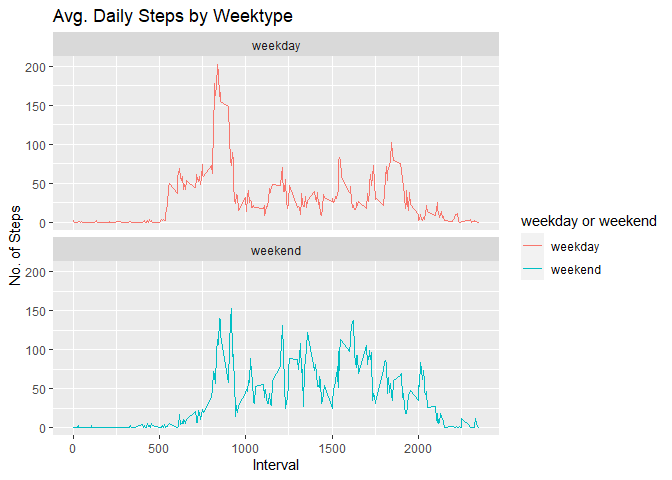
\includegraphics{Peer-graded_Assignment_files/figure-latex/unnamed-chunk-13-1.pdf}

\end{document}
